% !TeX program = lualatex

\documentclass[12pt]{article}



\usepackage[margin=1in]{geometry} 
\usepackage{amsmath,amsthm,amssymb}
\usepackage{MnSymbol}
\usepackage{graphicx}
\usepackage{bm}
\usepackage[normalem,normalbf]{ulem}
\usepackage{algorithm} 
\usepackage{algpseudocode} 
\usepackage{multirow}
\usepackage{rotating}
\usepackage{therefore}

\usepackage{tikz}
\usetikzlibrary{shapes.multipart}
\usetikzlibrary{shapes.symbols}

\usetikzlibrary{graphs,graphdrawing,graphs.standard,quotes}
\usegdlibrary{circular,force,layered,routing}
\tikzset{
	graphs/simpleer/.style={
		nodes={draw,circle, blue, left color=blue!20, text=black, inner sep=1pt},
		node distance=2.5cm, nodes={minimum size=2em}
	},
	every loop/.style={},
}

\newcommand*\circled[1]{\tikz[baseline=(char.base)]{
		\node[shape=circle,draw,inner sep=2pt] (char) {#1};}}

\newcommand{\m}{\medskip\\}
\newcommand{\N}{\mathbb{N}}
\newcommand{\Z}{\mathbb{Z}}
\newcommand{\R}{\mathbb{R}}
\newcommand{\bbs}{\textbackslash\textbackslash\space}
\newcommand{\bs}{\textbackslash\space}
\newcommand{\la}{\enskip\land\enskip}
\newcommand{\lo}{\enskip\lor\enskip}
\newcommand{\comp}[1]{#1^\mathsf{c}}
\newcommand{\micdrop}{\qed}
\newcommand{\contra}{\begin{tikzpicture}
		\node[starburst, draw, minimum width=3cm, minimum height=2cm,line width=1.5pt,red,fill=yellow,scale=.5]
		{BOOM, A CONTRADICTION!!!};
\end{tikzpicture}}

\renewcommand{\qedsymbol}{$\blacksquare$}

\DeclareMathOperator{\lcm}{lcm}

\newtheorem{theorem}{Theorem}

\newenvironment{exercise}[2][Exercise]{\begin{trivlist}
		\item[\hskip \labelsep {\bfseries #1}\hskip \labelsep {\bfseries #2.}]}{\end{trivlist}}

\setlength\parindent{24pt}

\makeatletter
\renewcommand*\env@matrix[1][*\c@MaxMatrixCols c]{%
	\hskip -\arraycolsep
	\let\@ifnextchar\new@ifnextchar
	\array{#1}}
\makeatother
\setlength\parindent{24pt}



\begin{document}
	
	% --------------------------------------------------------------
	%                         Start here
	% --------------------------------------------------------------
	
	
	\title{Homework 4 (Due Feb 8, 2023)}
	\author{Jack Hyatt\\ %replace with your name
		MATH 575 - Discrete Mathamatics II - Spring 2023} 
	
	\maketitle
	
	Justify all of your answers completely.\\
	
	
	\medskip 
	
\begin{enumerate}

\item Let $M$ be a maximum matching of a graph $G$, and let $M'$ be a {\em maximal} matching of $G$. Prove that $|M'| \geq \frac{|M|}{2}$. 

\begin{proof}
	Let $M$ be a maximum matching of a graph $G$, and let $M'$ be a {\em maximal} matching of $G$. Assume towards contradiction that $|M'| < \frac{|M|}{2}$. Let $e$ be an edge in $M'$. Since $M$ is maximum, then $M$ must contain at least one, and at most 2 edges incident to $e$, because otherwise we could add $e$ to $M$ and then $M$ wouldn't have been maximum. Let $a$ be the number of edges in $M$ that are incident to some saturated vertex in $M'$.\\
	So $a\leq2|M'|<|M| \implies a<|M|$. So then there is some edge $e'\in M$	that is not incident to any vertex in $M'$.\Therefore we should be able to add $e'$ to $M'$, meaning $M'$ wasn't maximal.\contra
\end{proof}

\medskip

\item Consider the following graph and the matching given by the edges $M = \{CE, BG, HI, KM\}$.

\begin{center}
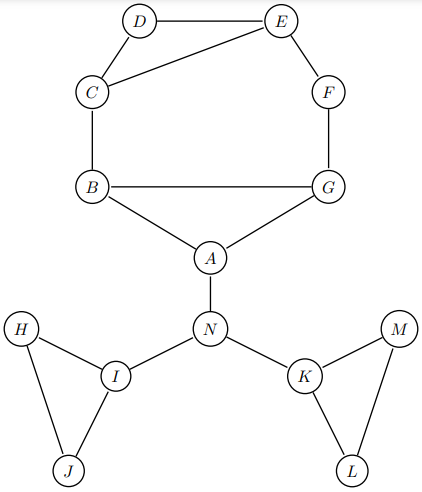
\includegraphics[scale=.5]{Q1.png}
\end{center}

\begin{enumerate}
\item Starting from the matching $M$, use a series of augmenting paths to find a matching in the graph of size 6. Write down the vertices for each augmenting path you use.\m
Starting with M, we see that $(D,E,C,B,G,A)$ is an augmenting path. So now our new matching is $M = \{DE,CB,GA,HI,KM\}$. Now we have $(F,E,D,C,B,G,A,N)$ is an augmenting path. Our new matching with 6 matches is now \\$M = \{FE,DC,BG,AN,HI,KM\}$.

\item Is the matching you found in part (a) maximum? If so, explain why. If not, find a larger matching.\m
Yes, because there are no augmenting paths left.
 
\end{enumerate}



\medskip

\item 6 instructors $i_1, i_2, \ldots, i_6$ must be assigned to teach 6 classes $c_1, c_2, \ldots, c_6$, 1 class per instructor. The table below shows an ``x" if a teacher has taught a class in a previous semester. Suppose each teacher would prefer to teach a class they have taught in the past. 
\begin{center}
\begin{tabular}{ |c|c|c|c|c|c|c| } 
 \hline
      & $c_1$ & $c_2$ & $c_3$ & $c_4$ & $c_5$ & $c_6$\\
\hline
$i_1$ &   x   &       &   x   &       &       &   x   \\
\hline
$i_2$ &       &   x   &       &       &       &       \\
\hline
$i_3$ &   x   &       &   x   &       &       &       \\
\hline
$i_4$ &       &       &       &   x   &   x   &       \\
\hline
$i_5$ &       &       &   x   &       &       &   x   \\
\hline
$i_6$ &       &       &   x   &       &       &   x   \\
\hline

\end{tabular}
\end{center}

\begin{enumerate}
\item Construct a bipartite graph $G$ such that a matching in $G$ corresponds to a (partial) assignment of instructors to classes.
\begin{center}
\tikz \graph [math nodes,grow right sep=2cm,nodes={circle,draw}]{ 
	subgraph I_nm [V={i_1,i_2,i_3,i_4,i_5,i_6}, 
	W={c_1,c_2,c_3,c_4,c_5,c_6}];
	
	i_1 -- {c_1,c_3,c_6};
	i_2 -- {c_2};
	i_3 -- {c_1,c_3};
	i_4 -- {c_4,c_5};
	i_5 -- {c_3,c_6};
	i_6 -- {c_3,c_6};
	};
\end{center}
\item Find a maximum matching of $G$ from part(a). Can every instructor be assigned a class of their preference? If not, find a subset of the instructors that violate Hall's condition.\m
The set $\{i_1,i_3,i_5,i_6\}$ has $\{c_1,c_3,c_6\}$ as neighbors, a subset that violates Hall's condition.
\end{enumerate}

\medskip 
\item In a bipartite graph $G = X \cupdot Y$, the {\em deficiency} of a set $S \subseteq X$ is \[\operatorname{def}(S) = \max\{0, |S| - |N(S)|\}.\] Prove that a maximum matching in $G$ has size $|X| - \max_{S \subseteq X} \operatorname{def}(S)$.
\begin{proof}
	Let $G = X \cupdot Y$ be a bipartite graph. WLOG, let $|X|\geq |Y|$. Let us construct a graph $G'$ with the following rules: $G'$ is the same as $G$, except we add vertices to $Y$ in a certain way. The set of vertices we will add shall be called $W$. $|W| = \max_{S \subseteq X} \operatorname{def}(S)$, and $W$ and $X$ form a complete bipartite subgraph.\par
	This graph $G'$ has a matching that saturates $X$ iff $G$ has a matching of size $|X| - \max_{S \subseteq X} \operatorname{def}(S)$. This is true because if $G$ has a matching of the desired size, then there are $\max_{S \subseteq X} \operatorname{def}(S)$ vertices in $X$ unmatched, which then can be matched to vertices in $W$. If $G'$ has a matching saturating $X$, with how we constructed $G'$, taking away $W$ from $G'$ leaves $\max_{S \subseteq X} \operatorname{def}(S)$ vertices in $X$ unmatched, meaning $G$ has a matching of the desired size.\par
	We know $G'$ always saturates $X$ because the max deficiency finds the subset with the greatest difference in vertices with its neighbor vertices, which would leave $|S| - |N(S)|$ unmatched vertices in $X$ in any maximum matching. So the addition of $W$ to $Y$ makes it so that every vertex in $X$ can be match, fully saturating $X$. \Therefore $X$ is always fully saturated in $G'$, meaning $G$ has a matching of the desired size always.
\end{proof}


\medskip

\item For $d \in \mathbb N$, the $d$-dimensional hypercube $Q_d$ is the $2^d$-vertex graph in which every vertex is a binary string of length $d$, and two vertices are adjacent if their corresponding strings differ in exactly one coordinate. 

  Prove that for $d \geq 2$, $Q_d$ has at least $2^{2^{d-2}}$ perfect matchings. 
\begin{center}
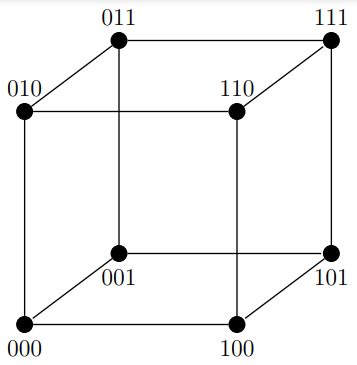
\includegraphics[scale=.5]{Q3.png}
\end{center}
\begin{proof}
	We shall induct on the number of dimensions, $d$, to show the above fact.\\
	\textbf{Base Case}: d=2\\
	It is clear that a $Q_2 = C_4$ which has $2 = 2^1 = 2^{2^{2-2}}$ perfect matchings.\\
	Induction Step: Let $d\geq2$ and $Q_d$ have $2^{2^{d-2}}$ perfect matchings.\\ 
	Consider the $d+1$ case. $Q_{d+1}$ is created by making two $Q_d$'s, and putting a 0 in front of the vertices of one, and a 1 in front of the vertices of the other. Before connecting these two components through the rule, we see that each component has $2^{2^{d-2}}$ perfect matchings. So a lower bound for the total perfect matchings for $Q_{d+1}$ is to use the multiplication rule of combinatorics and multiply $2^{2^{d-2}}\cdot2^{2^{d-2}} = (2^{2^{d-2}})^2 = 2^{2\cdot2^{d-2}} = 2^{2^{d-1}}$.\\
	\Therefore by P.M.I., $Q_d$ has at least $2^{2^{d-2}}$ perfect matchings.
\end{proof}
\end{enumerate}
\vspace{3cm} I have a LaTeX package that has a Therefore command that will give a random funny phrase that is similar to the word therefore, fyi.
\end{document}
